Тестування відбувалося на машині із процесором Intel Core i7-8550U 1.99GHz під 64-бітною версією операційної системи Windows.

\section{Перша задача, неадаптивні алгоритми}

Для усіх алгоритмів у якості початкового наближення ми брали $x_1 = (1, \dots, 1)$, $\epsilon = 10^{-3}$, $\lambda = 0.4$ (константа Ліпшиця цієї задачі дорівнює одиниці: $L = 1$). 

\begin{figure}[H]
    \centering
    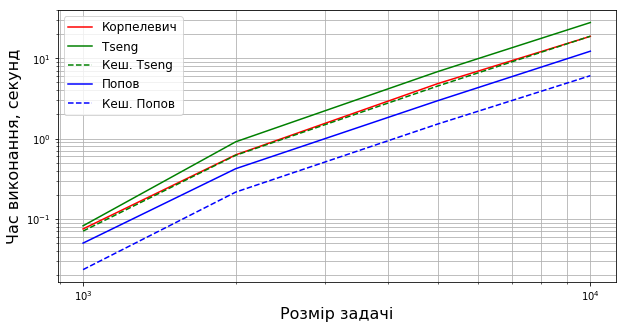
\includegraphics[width=\textwidth]{img/1/time.png}
    \caption{Результати неадаптивних алгоритмів на першій задачі}
\end{figure}

І справді, бачимо що алгоритм Корпелевич і кешований алгоритм Tseng'a справді показують майже однакові результати, а також обидві некешовані версії програють кешованим. Та сама інформація у табличці, для зручності:

\begin{table}[H]
	\centering
	\begin{tabular}{|c||c|c|c|c|}\hline
		Розмір задачі & 1000 & 2000 & 5000 & 10000 \\ \hline \hline
		Корпелевич & 0.11 & 0.65 & 4.95 & 19.31 \\ \hline
		Tseng & 0.10 & 0.98 & 7.13 & 26.82 \\ \hline
		Кеш. Tseng & 0.07 & 0.71 & 4.49 & 17.98 \\ \hline
		Попов & 0.08 & 0.50 & 2.98 & 12.18 \\ \hline
		Кеш. Попов & 0.03 & 0.26 & 1.52 & 6.16 \\ \hline
	\end{tabular}
	\caption{Час виконання, секунд}
\end{table}


\begin{table}[H]
	\centering
	\begin{tabular}{|c||c|c|c|c|}\hline
		Розмір задачі & 1000 & 2000 & 5000 & 10000 \\ \hline \hline
		Корпелевич & 132 & 137 & 144 & 148 \\ \hline
		Tseng & 132 & 137 & 144 & 148 \\ \hline
		Попов & 89 & 92 & 96 & 99 \\ \hline
		Маліцький Tam & 91 & 94 & 98 & 101 \\ \hline
	\end{tabular}
	\caption{Число ітерацій}
\end{table}


\section{Перша задача, адаптивні алгоритми}

\begin{figure}[H]
    \centering
    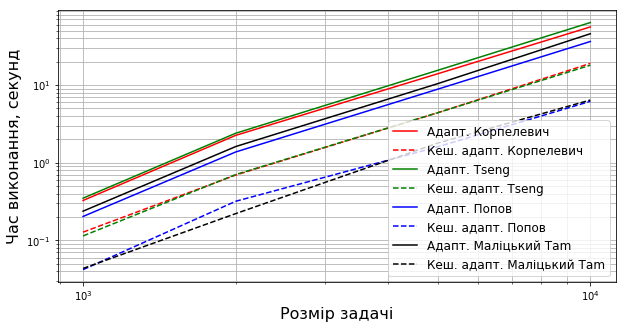
\includegraphics[width=\textwidth]{img/1/adapt/time.png}
    \caption{Результати адаптивних алгоритмів на першій задачі}
\end{figure}

Та сама інформація у табличці, для зручності:

\begin{table}[H]
	\centering
	\begin{tabular}{|c||c|c|c|c|}\hline
		Розмір задачі & 1000 & 2000 & 5000 & 10000 \\ \hline \hline
		Корпелевич & 0.11 & 0.65 & 4.95 & 19.31 \\ \hline
		Tseng & 0.10 & 0.98 & 7.13 & 26.82 \\ \hline
		Кеш. Tseng & 0.07 & 0.71 & 4.49 & 17.98 \\ \hline
		Попов & 0.08 & 0.50 & 2.98 & 12.18 \\ \hline
		Кеш. Попов & 0.03 & 0.26 & 1.52 & 6.16 \\ \hline \hline
		Адапт. Корпелевич & 0.21 & 1.71 & 12.70 & 50.57 \\ \hline
		Кеш. адапт. Корпелевич & 0.11 & 0.56 & 4.15 & 16.89 \\ \hline
		Адапт. Tseng & 0.27 & 1.91 & 14.58 & 58.36 \\ \hline
		Кеш. адапт. Tseng & 0.07 & 0.57 & 4.16 & 16.69 \\ \hline
		Адапт. Попов & 0.31 & 2.45 & 17.84 & 73.44 \\ \hline
		Кеш. адапт. Попов & 0.07 & 0.54 & 3.03 & 12.29 \\ \hline
	\end{tabular}
	\caption{Час виконання, секунд}
\end{table}


Алгоритма Попова програє своїй неадаптивній версії. Окрім цього, некешовані версії адаптивних алгоритмів явно програють кешованим. Кешовані версії адаптивних алгоритмів Корпелевич і Tseng'a не поступаються кешованим неадаптивним версіям. \medskip

Щодо кількості ітерацій ситуація схожа:

\begin{table}[H]
	\centering
	\begin{tabular}{|c||c|c|c|c|}\hline
		Розмір задачі & 1000 & 2000 & 5000 & 10000 \\ \hline \hline
		Адапт. Корпелевич & 125 & 129 & 135 & 139 \\ \hline
		Кеш. адапт. Корпелевич & 125 & 129 & 135 & 139 \\ \hline
		Адапт. Tseng & 125 & 129 & 135 & 139 \\ \hline
		Кеш. адапт. Tseng & 125 & 129 & 135 & 139 \\ \hline
		Адапт. Попов & 179 & 185 & 194 & 201 \\ \hline
		Кеш. адапт. Попов & 179 & 185 & 194 & 201 \\ \hline
	\end{tabular}
	\caption{Число ітерацій}
\end{table}


\section{Перша задача із розрідженими матрицями, неадаптивні алгоритми}

Нескладно помітити, що матриця $A$ дуже розріджена, що наводить на ідею скористатися модулем scipy.sparse для ефективної роботи з розрідженими матрицями. Це дозволить нам розв'язувати задачу для значно більших $m$.

\begin{figure}[H]
    \centering
    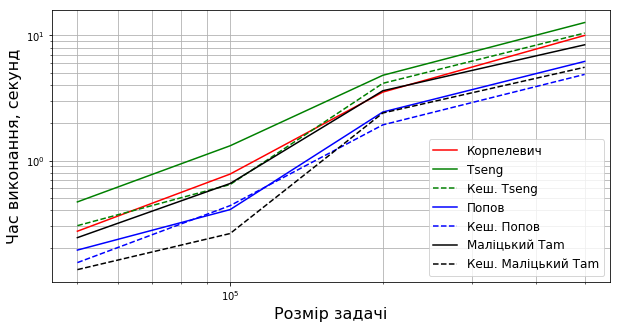
\includegraphics[width=\textwidth]{img/1/sparse/time.png}
    \caption{Результати неадаптивних алгоритмів на першій задачі із розрідженими матрицями}
\end{figure}

Та сама інформація у табличці, для зручності:

\begin{table}[H]
	\centering
	\begin{tabular}{|c||c|c|c|c|}\hline
		Розмір задачі & 50000 & 100000 & 200000 & 500000 \\ \hline \hline
		Корпелевич & 0.06 & 0.24 & 2.04 & 3.56 \\ \hline
		Tseng & 0.08 & 0.38 & 1.78 & 5.56 \\ \hline
		Кеш. Tseng & 0.07 & 0.21 & 1.35 & 5.22 \\ \hline
		Попов & 0.04 & 0.10 & 1.03 & 2.82 \\ \hline
		Кеш. Попов & 0.03 & 0.13 & 1.13 & 2.73 \\ \hline
	\end{tabular}
	\caption{Час виконання, секунд}
\end{table}


\begin{table}[H]
	\centering
	\begin{tabular}{|c||c|c|c|c|}\hline
		Розмір задачі & 50000 & 100000 & 200000 & 500000 \\ \hline \hline
		Корпелевич & 255 & 260 & 265 & 271 \\ \hline
		Tseng & 255 & 260 & 265 & 271 \\ \hline
		Кеш. Tseng & 255 & 260 & 265 & 271 \\ \hline
		Попов & 168 & 171 & 174 & 178 \\ \hline
		Кеш. Попов & 168 & 171 & 174 & 178 \\ \hline
		Маліцький Tam & 170 & 173 & 176 & 180 \\ \hline
		Кеш. Маліцький Tam & 170 & 173 & 176 & 180 \\ \hline
	\end{tabular}
	\caption{Число ітерацій}
\end{table}


\begin{remark}
    Тут перевага кешування вже не така очевидна, адже ми значно здешевили обчислення оператора $A$, хоча все ще присутня.
\end{remark}

\section{Перша задача із розрідженими матрицями, адаптивні алгоритми}

\begin{figure}[H]
    \centering
    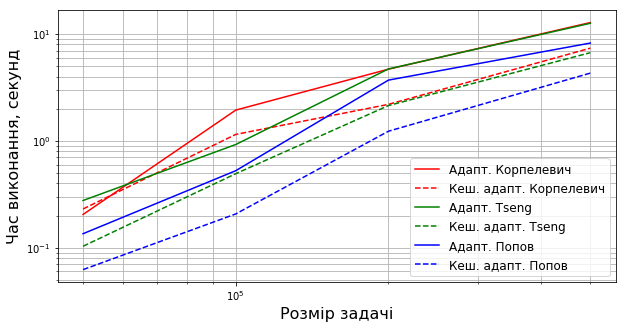
\includegraphics[width=\textwidth]{img/1/sparse/adapt/time.png}
    \caption{Результати адаптивних алгоритмів на першій задачі із розрідженими матрицями}
\end{figure}

Та сама інформація у табличці:

\begin{table}[H]
	\centering
	\begin{tabular}{|c||c|c|c|c|}\hline
		Розмір задачі & 50000 & 100000 & 200000 & 500000 \\ \hline \hline
		Корпелевич & 0.07 & 0.23 & 2.23 & 5.28 \\ \hline
		Tseng & 0.13 & 0.53 & 1.96 & 6.97 \\ \hline
		Кеш. Tseng & 0.09 & 0.24 & 1.75 & 5.69 \\ \hline
		Попов & 0.06 & 0.12 & 1.58 & 3.91 \\ \hline
		Кеш. Попов & 0.04 & 0.25 & 0.86 & 2.09 \\ \hline
		Маліцький Tam & 0.07 & 0.26 & 1.33 & 5.09 \\ \hline
		Кеш. Маліцький Tam & 0.04 & 0.10 & 0.91 & 3.76 \\ \hline \hline
		Адапт. Корпелевич & 0.27 & 0.95 & 4.85 & 13.73 \\ \hline
		Кеш. адапт. Корпелевич & 0.11 & 1.07 & 2.41 & 7.64 \\ \hline
		Адапт. Tseng & 0.20 & 1.20 & 4.65 & 14.15 \\ \hline
		Кеш. адапт. Tseng & 0.11 & 0.62 & 3.19 & 7.31 \\ \hline
		Адапт. Попов & 0.24 & 0.68 & 3.54 & 9.67 \\ \hline
		Кеш. адапт. Попов & 0.07 & 0.17 & 2.14 & 4.35 \\ \hline
		Адапт. Маліцький Tam & 0.14 & 0.37 & 3.14 & 9.35 \\ \hline
		Кеш. адапт. Маліцький Tam & 0.09 & 0.13 & 1.81 & 4.73 \\ \hline
	\end{tabular}
	\caption{Час виконання, секунд}
\end{table}


\begin{table}[H]
	\centering
	\begin{tabular}{|c||c|c|c|c|}\hline
		Розмір задачі & 50000 & 100000 & 200000 & 500000 \\ \hline \hline
		Адапт. Корпелевич & 256 & 261 & 266 & 272 \\ \hline
		Кеш. адапт. Корпелевич & 256 & 261 & 266 & 272 \\ \hline
		Адапт. Tseng & 256 & 261 & 266 & 272 \\ \hline
		Кеш. адапт. Tseng & 224 & 229 & 234 & 240 \\ \hline
		Адапт. Попов & 149 & 152 & 155 & 159 \\ \hline
		Кеш. адапт. Попов & 149 & 152 & 155 & 159 \\ \hline
		Адапт. Маліцький Tam & 171 & 175 & 178 & 182 \\ \hline
		Кеш. адапт. Маліцький Tam & 171 & 175 & 178 & 182 \\ \hline
	\end{tabular}
	\caption{Число ітерацій}
\end{table}


Ситуація доволі схожа на попередню, за виключення того що алгоритм Попва тепер не так суттєво програє неадаптивній версії.

\section{Друга задача, неадаптивні алгоритми}

Для кожного алгоритму і кожного розміру задачі було проведено $5$ запусків (із різними матрицями), у таблиці і на графіку наведені середні значення та середньоквадратичні відхилення.

\begin{figure}[H]
    \centering
    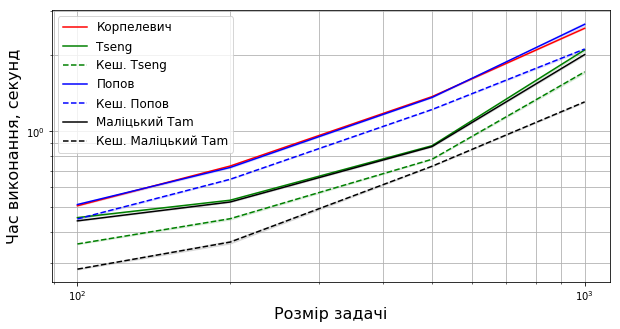
\includegraphics[width=\textwidth]{img/2/time.png}
    \caption{Результати неадаптивних алгоритмів на другій задачі}
\end{figure}

Та сама інформація у табличці, для зручності:

\begin{table}[H]
	\centering
	\begin{tabular}{|c||c|c|c|c|}\hline
		Розмір задачі & 100 & 200 & 500 & 1000 \\ \hline \hline
		Корпелевич & 0.54 $\pm$ 0.27 & 0.87 $\pm$ 0.30 & 2.39 $\pm$ 0.52 & 7.62 $\pm$ 0.59 \\ \hline
		Tseng & 0.48 $\pm$ 0.27 & 0.77 $\pm$ 0.21 & 1.85 $\pm$ 0.37 & 6.36 $\pm$ 0.77 \\ \hline
		Кеш. Tseng & 0.38 $\pm$ 0.20 & 0.72 $\pm$ 0.11 & 1.40 $\pm$ 0.55 & 4.95 $\pm$ 0.75 \\ \hline
		Попов & 0.49 $\pm$ 0.18 & 1.16 $\pm$ 0.32 & 2.25 $\pm$ 0.69 & 7.79 $\pm$ 1.08 \\ \hline
		Кеш. Попов & 0.34 $\pm$ 0.16 & 0.86 $\pm$ 0.36 & 2.45 $\pm$ 0.40 & 6.39 $\pm$ 0.64 \\ \hline
		Маліцький Tam & 0.49 $\pm$ 0.17 & 0.56 $\pm$ 0.16 & 1.49 $\pm$ 0.48 & 6.10 $\pm$ 0.90 \\ \hline
		Кеш. Маліцький Tam & 0.29 $\pm$ 0.09 & 0.34 $\pm$ 0.06 & 1.19 $\pm$ 0.48 & 3.85 $\pm$ 0.44 \\ \hline
	\end{tabular}
	\caption{Час виконання, секунд}
\end{table}


У цій задачі основна складність все ще у обчисленні оператора $A$, %($O(m^2)$)
хоча обчислення проекції вже більш складне, %($O(m \log m)$)
тому алгоритм Tseng'a має певну перевагу над алгоритмом Попова, який у свою чергу випереджає алгоритм Корпелевич. Щодо кількості ітерацій то усі три алгоритми демонструють практично ідентичні результати.

\begin{table}[H]
	\centering
	\begin{tabular}{|c||c|c|c|c|}\hline
		Розмір задачі & 100 & 200 & 500 & 1000 \\ \hline \hline
		Корпелевич & 1000 $\pm$ 0 & 1000 $\pm$ 0 & 1000 $\pm$ 0 & 1000 $\pm$ 0 \\ \hline
		Tseng & 1000 $\pm$ 0 & 1000 $\pm$ 0 & 1000 $\pm$ 0 & 1000 $\pm$ 0 \\ \hline
		Кеш. Tseng & 1000 $\pm$ 0 & 1000 $\pm$ 0 & 1000 $\pm$ 0 & 1000 $\pm$ 0 \\ \hline
		Попов & 1000 $\pm$ 0 & 1000 $\pm$ 0 & 1000 $\pm$ 0 & 1000 $\pm$ 0 \\ \hline
		Кеш. Попов & 1000 $\pm$ 0 & 1000 $\pm$ 0 & 1000 $\pm$ 0 & 1000 $\pm$ 0 \\ \hline
		Маліцький Tam & 1000 $\pm$ 0 & 1000 $\pm$ 0 & 1000 $\pm$ 0 & 1000 $\pm$ 0 \\ \hline
		Кеш. Маліцький Tam & 1000 $\pm$ 0 & 1000 $\pm$ 0 & 1000 $\pm$ 0 & 1000 $\pm$ 0 \\ \hline
	\end{tabular}
	\caption{Число ітерацій}
\end{table}


Знову ж таки, кешування дає перевагу на великих задачах, хоча вона вже не у 1.5--2 рази.

\begin{remark}
    Можна додати якийсь із матрчиних розкладів $M$ для пришвидшення множення $M x$. 
\end{remark}

\section{Друга задача, адаптивні алгоритми}

\begin{figure}[H]
    \centering
    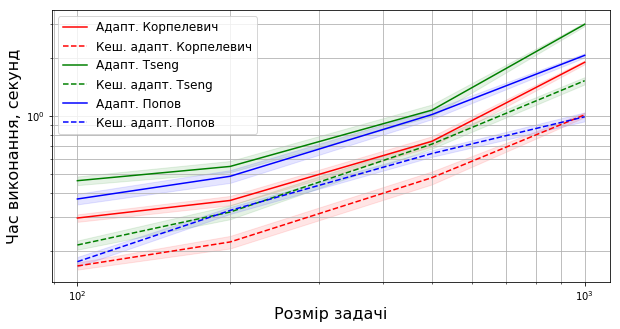
\includegraphics[width=\textwidth]{img/2/adapt/time.png}
    \caption{Результати адаптивних алгоритмів на другій задачі}
\end{figure}

Та сама інформація у табличці:

\begin{table}[H]
	\centering
	\begin{tabular}{|c||c|c|c|c|}\hline
		Розмір задачі & 100 & 200 & 500 & 1000 \\ \hline \hline
		Адапт. Корпелевич & 0.69 $\pm$ 0.12 & 0.99 $\pm$ 0.13 & 1.70 $\pm$ 0.10 & 3.79 $\pm$ 0.15 \\ \hline
		Кеш. адапт. Корпелевич & 0.42 $\pm$ 0.08 & 0.68 $\pm$ 0.10 & 1.39 $\pm$ 0.07 & 2.56 $\pm$ 0.07 \\ \hline
		Адапт. Tseng & 0.86 $\pm$ 0.02 & 0.98 $\pm$ 0.01 & 1.42 $\pm$ 0.02 & 3.08 $\pm$ 0.11 \\ \hline
		Кеш. адапт. Tseng & 0.49 $\pm$ 0.09 & 0.80 $\pm$ 0.07 & 1.72 $\pm$ 0.19 & 3.49 $\pm$ 0.29 \\ \hline
		Адапт. Попов & 0.82 $\pm$ 0.19 & 1.19 $\pm$ 0.18 & 2.12 $\pm$ 0.33 & 4.78 $\pm$ 0.51 \\ \hline
		Кеш. адапт. Попов & 0.45 $\pm$ 0.09 & 0.76 $\pm$ 0.11 & 1.46 $\pm$ 0.19 & 2.65 $\pm$ 0.28 \\ \hline
		Адапт. Маліцький Tam & 0.87 $\pm$ 0.02 & 0.99 $\pm$ 0.03 & 1.39 $\pm$ 0.03 & 3.02 $\pm$ 0.02 \\ \hline
		Кеш. адапт. Маліцький Tam & 0.33 $\pm$ 0.02 & 0.45 $\pm$ 0.01 & 0.79 $\pm$ 0.01 & 1.35 $\pm$ 0.00 \\ \hline
	\end{tabular}
	\caption{Час виконання, секунд}
\end{table}


Адаптивні версії суттєво випереджають неадаптивні, причому за числом ітерацій також:

\begin{table}[H]
	\centering
	\begin{tabular}{|c||c|c|c|c|}\hline
		Розмір задачі & 100 & 200 & 500 & 1000 \\ \hline \hline
		Адапт. Корпелевич & 317 $\pm$ 66 & 359 $\pm$ 42 & 410 $\pm$ 34 & 451 $\pm$ 46 \\ \hline
		Адапт. Tseng & 504 $\pm$ 50 & 684 $\pm$ 38 & 872 $\pm$ 73 & 994 $\pm$ 68 \\ \hline
		Адапт. Попов & 430 $\pm$ 93 & 507 $\pm$ 64 & 551 $\pm$ 48 & 606 $\pm$ 57 \\ \hline
		Адапт. Маліцький Tam & 540 $\pm$ 93 & 599 $\pm$ 70 & 633 $\pm$ 52 & 647 $\pm$ 42 \\ \hline
	\end{tabular}
	\caption{Число ітерацій}
\end{table}


\section{Четверта задача, адаптивні алгоритми}

А цій задачі константа Ліпшиця мені невідома, тому тут наводяться результати лише адаптивних алгоритмів.

\begin{figure}[H]
    \centering
    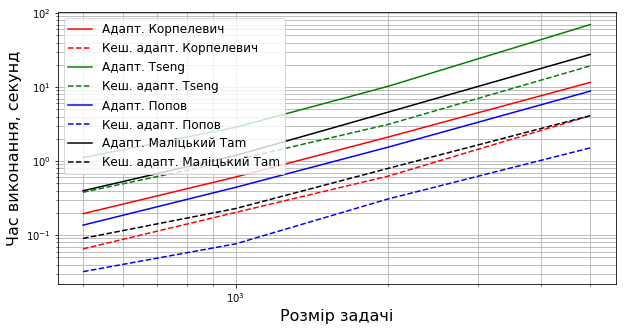
\includegraphics[width=\textwidth]{img/4/adapt/time.png}
    \caption{Результати адаптивних алгоритмів на четвертій задачі}
\end{figure}

Та сама інформація у табличці:

\begin{table}[H]
	\centering
	\begin{tabular}{|c||c|c|c|c|}\hline
		Розмір задачі & 500 & 1000 & 2000 & 5000 \\ \hline \hline
		Адапт. Корпелевич & 0.19 & 0.61 & 2.12 & 11.56 \\ \hline
		Кеш. адапт. Корпелевич & 0.07 & 0.20 & 0.63 & 4.10 \\ \hline
		Адапт. Tseng & 1.11 & 2.86 & 10.27 & 69.95 \\ \hline
		Кеш. адапт. Tseng & 0.38 & 1.04 & 3.14 & 19.33 \\ \hline
		Адапт. Попов & 0.14 & 0.44 & 1.55 & 8.82 \\ \hline
		Кеш. адапт. Попов & 0.03 & 0.08 & 0.31 & 1.51 \\ \hline
		Адапт. Маліцький Tam & 0.40 & 1.19 & 4.60 & 27.66 \\ \hline
		Кеш. адапт. Маліцький Tam & 0.09 & 0.23 & 0.80 & 4.11 \\ \hline
	\end{tabular}
	\caption{Число ітерацій}
\end{table}


\begin{table}[H]
	\centering
	\begin{tabular}{|c||c|c|c|c|}\hline
		Розмір задачі & 500 & 1000 & 2000 & 5000 \\ \hline \hline
		Адапт. Корпелевич & 111 & 113 & 116 & 119 \\ \hline
		Адапт. Tseng & 558 & 572 & 587 & 605 \\ \hline
		Адапт. Попов & 87 & 89 & 91 & 94 \\ \hline
	\end{tabular}
	\caption{Число ітерацій}
\end{table}


\section{Четверта задача  із розрідженими матрицями, адаптивні алгоритми}

\begin{figure}[H]
    \centering
    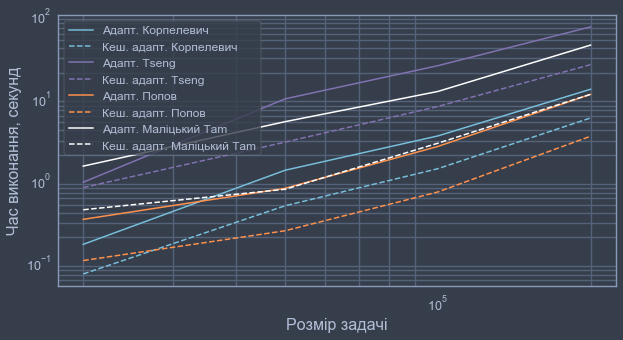
\includegraphics[width=\textwidth]{img/4/sparse/adapt/time.png}
    \caption{Результати адаптивних алгоритмів на четвертій задачі із розрідженими матрицями}
\end{figure}

Та сама інформація у табличці:

\begin{table}[H]
	\centering
	\begin{tabular}{|c||c|c|c|c|}\hline
		Розмір задачі & 20000 & 50000 & 100000 & 200000 \\ \hline \hline
		Адапт. Корпелевич & 0.14 & 1.14 & 1.88 & 8.93 \\ \hline
		Кеш. адапт. Корпелевич & 0.07 & 0.45 & 0.96 & 3.87 \\ \hline
		Адапт. Tseng & 1.19 & 4.66 & 10.80 & 54.18 \\ \hline
		Кеш. адапт. Tseng & 0.75 & 1.73 & 3.76 & 19.40 \\ \hline
		Адапт. Попов & 0.34 & 0.59 & 2.39 & 7.84 \\ \hline
		Кеш. адапт. Попов & 0.11 & 0.13 & 0.57 & 2.75 \\ \hline
	\end{tabular}
	\caption{Час виконання, секунд}
\end{table}


\begin{table}[H]
	\centering
	\begin{tabular}{|c||c|c|c|c|}\hline
		Розмір задачі & 20000 & 50000 & 100000 & 200000 \\ \hline \hline
		Адапт. Корпелевич & 74 & 76 & 77 & 79 \\ \hline
		Адапт. Tseng & 388 & 399 & 408 & 416 \\ \hline
		Адапт. Попов & 71 & 73 & 74 & 76 \\ \hline
	\end{tabular}
	\caption{Число ітерацій}
\end{table}

